% !TeX root = Protokoll.tex
\begin{figure}[h!]
\centering
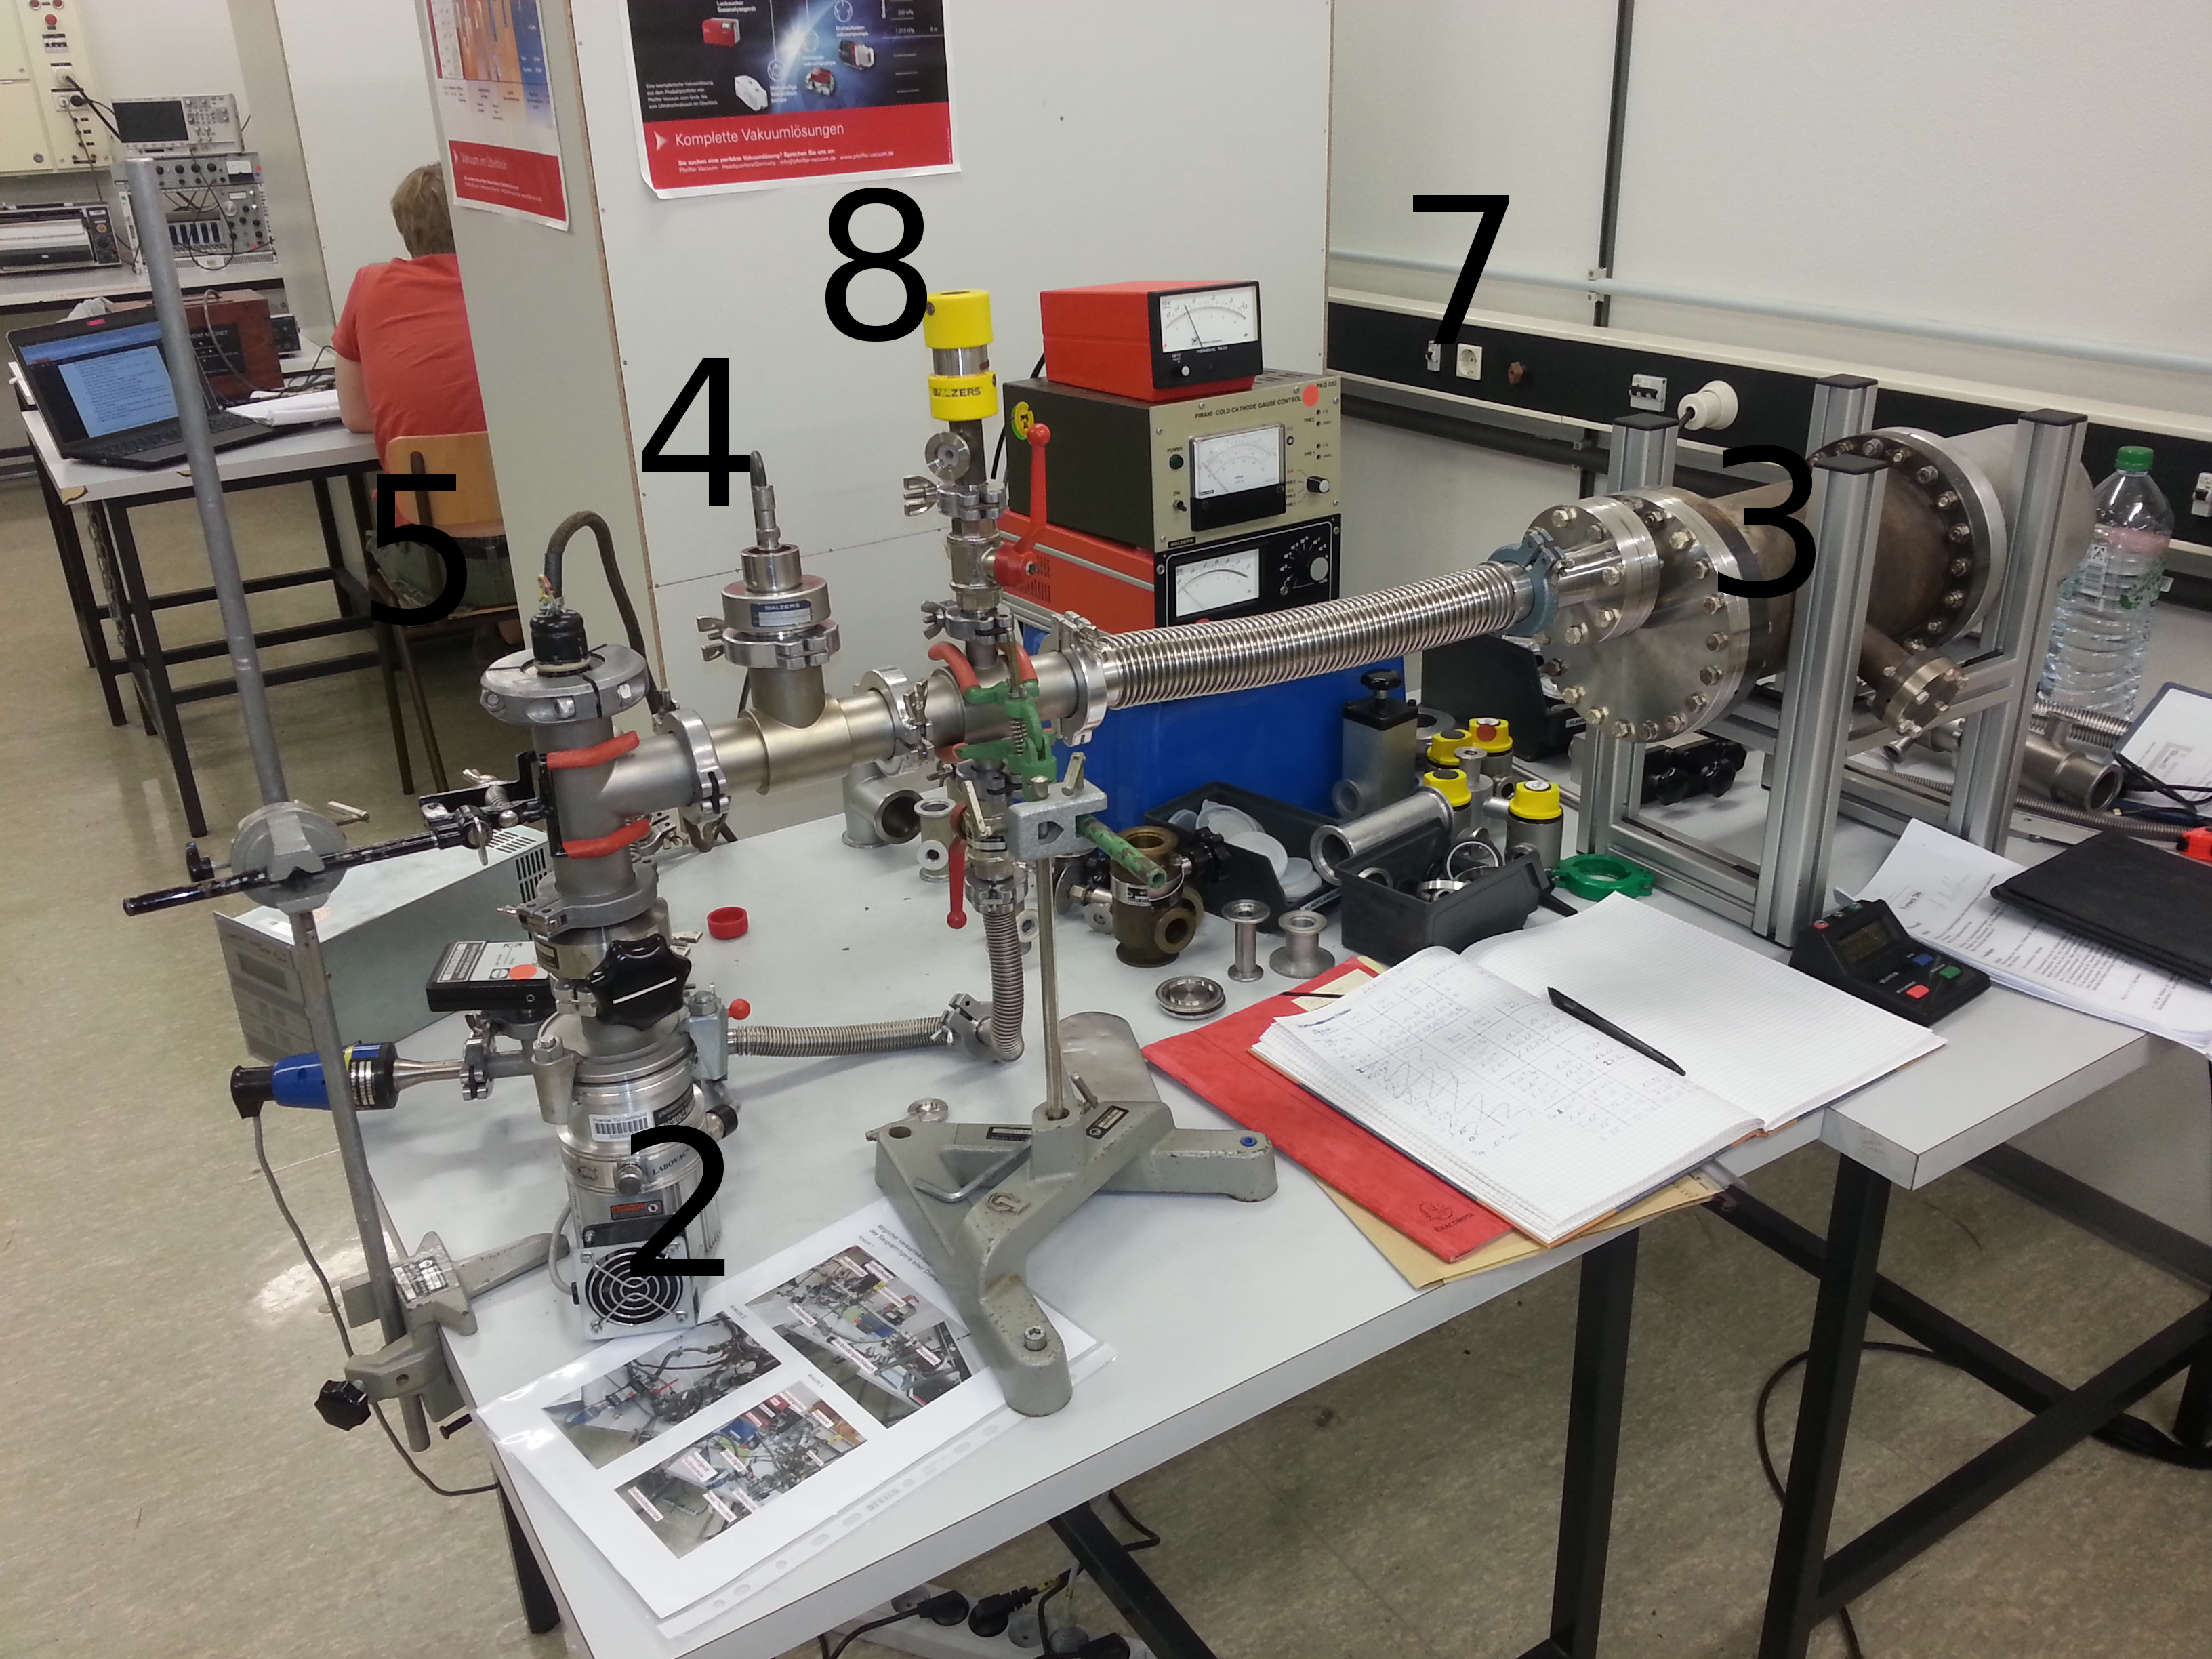
\includegraphics[scale=0.06]{../Grafiken/Aufbau_.jpg}
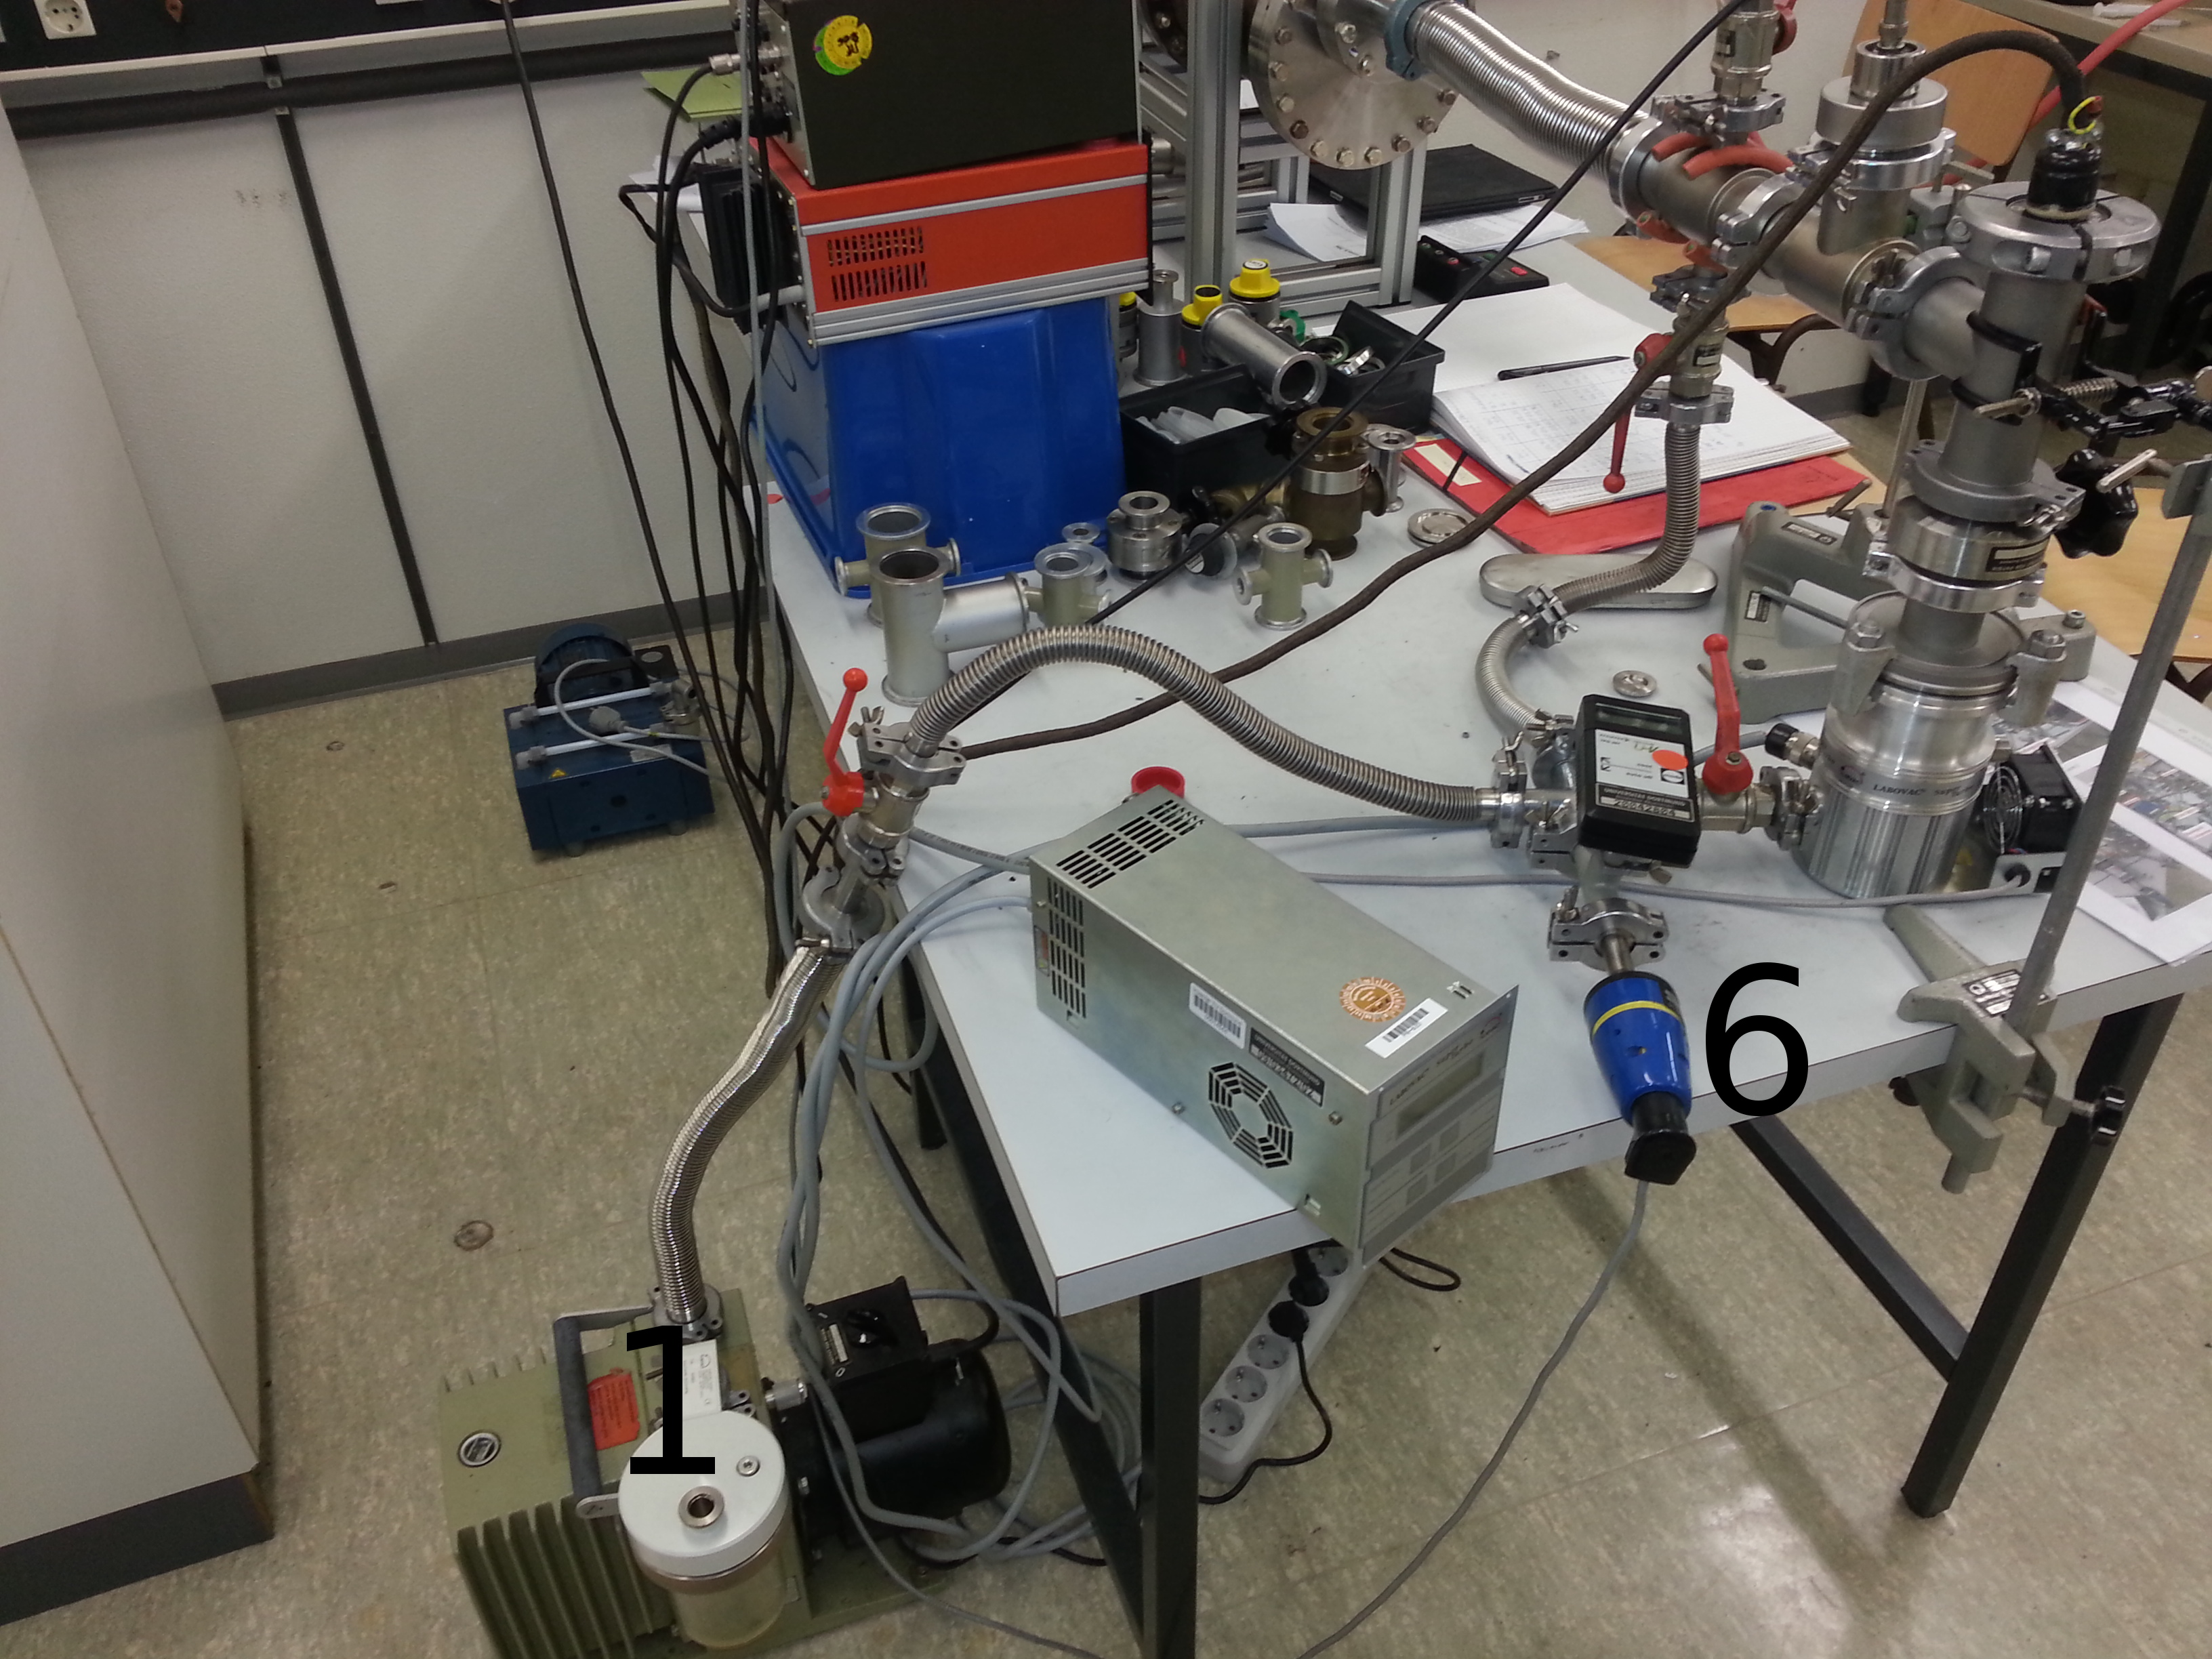
\includegraphics[scale=0.06]{../Grafiken/Drehschieber_.jpg}
\caption{Der Verwendete Aufbau aus zwei verschiedenen Winkeln.\label{fig:Aufbau}}
\end{figure}
Es werden so wohl eine Drehschieberpumpe (1) als auch eine Turbopumpe (2) mithilfe von Rohren und Ventilen an den Rezipienten (3) angeschlossen, wie in Abbildung \ref{fig:Aufbau} zu sehen.
Es befinden sich je ein Kaltkathoden- (4), Heißkathoden- (5) und Pirani-Vakuummeter (6) im Aufbau und die dazugehörigen Anzeigen (7), dabei wurde das digitale Messgerät zwar verbaut aber nicht für die Messung verwendet.
Weiter befinden sich mehre Ventile im Aufbau, um zum einem die Pumpen auszukoppeln und zum anderen verschiedene Bereiche vom Rezipienten zu trennen. Im Aufbau ist noch ein Belüftungsventil (8), mit dem das Volumen mit Luft gefüllt werden kann, an diesem kann ein Maß für ein Leck eingestellt werden.
Dabei ist darauf zu achten, dass mithilfe von Abdichtringen und Spannringen alle Verbindungen abgedichtet sind.
Vor der Messung wird einmal mithilfe der Drehschieberpumpe  das innere des Aufbaus ausgepumpt, über eine längere Zeit, damit unter anderem \glqq Wasserablagerungen\grqq{} entfernt werden. Bei einem Druck unter \SI{e-1}{\milli\bar}, kann die Turbopumpe ebenfalls angeschaltet werden. Dabei kann gleichzeitig überprüft werden, ob der Aufbau auch im Hochvakuum dicht ist.
\subsection{Saugvermögen}
Das Saugvermögen wird für beide Pumpen auf zwei Methoden bestimmt, einmal mithilfe der Evakuierungskurve und der Leckratenmessung.
\subsubsection{Evakuierungskurve der Drehschieberpumpe}
Zu Bestimmung der Evakuierungskurve, wird während die Pumpe Angeschaltet ist der Rezipient belüftet. Nach dem das Belüftungsventil geschlossen wurde kann die Zeit in Abhängigkeit des Drucks bestimmt werden. 
Weil das Vakuum ein Grobvakuum ist, wird hier mit dem Piani-Vakuummeter gearbeitet.
\subsubsection{Leckratenmessung für die Drehschieberpumpe}
Zunächst wird ein Leck am Belüftungsventil eingestellt, dann wird mithilfe der Drehschieberpumpe bis zum Ausgleichsdruck der Aufbau ausgepumpt. Nach dem Schließen des Ventils vor der Pumpe, kann der Druckanstieg gegen die Zeit gemessen werden. 
\subsubsection{Evakuierungskurve der Turbopumpe}
Die Messung für die Turbopumpe funktioniert wie bei der Drehschieberpumpe, allerdings muss zuerst ein Hochvakuum erzeugt werden. Dazu wird mithilfe der Drehschieberpumpe ein Vakuum von \SI{e-1}{\milli\bar} hergestellt, ab diesem Druck kann das Kaltkathoden-Vakuummeter verwendet werden und die Turbopumpe eingestellt werden. Der Druck wird auf unter \SI{5e-3}{\milli\bar} abgepumpt. Ab hier kann das Heißkathoden-Vakuummeter verwendet werden. Mit dem Belüftungsventil kann ein Ausgleichsdruck in Größenordnung von \SI{5e-3}{\milli\bar} eingestellt werden, in dem ein kleines Leck eingestellt wird. Durch Schließen des Belüftungsventils, kann der Druckabfall gegen die Zeit gemessen werden.
\subsubsection{Leckratenmessung der Turbopumpe}
Die Leckratenmessung läuft analog, zur der Messung bei der Drehschieber Pumpe. Nach dem Einstellen eines Ausgleichsdrucks, mit einem kleinen Leck wird das Ventil vor der Turbopumpe geschlossen und es wird der Druckanstieg mit der Zeit gemessen.
\subsection{Bestimmung des Volumens $V_0$}
Nach dem die Messreihen beendet wurden, muss das gesamt innen Volumen des Aufbaues bestimmt werden. Dazu wird jedes Bauteil einzeln vermessen.